\chapter{System design}

\textit{This chapter describes the process of designing our implementation. We divide our work into creating an open-source library that can help developers handle the primary function of a HD wallet (key generation, transaction integration, balance checking, etc.) and a Web Wallet for cryptocurrency users. }

\minitoc

\section{The Library}
Our work does not only share an identical problem with the problem statement. We realize that we could do better. With the support of SatoshiLabs proposal number 44 (BIP44), we can create wallets that hold multiple native tokens of different blockchains. We decided our HD wallet will support the blockchain using ed25519 as well as secp259k1 (two famous curves of the blockchain community). They are Bitcoin, Ethereum, and Solana. As we researched, there are almost no non-custodial hot wallets that support different kinds of coin holders. Even the existing libraries limit their support to a specific blockchain.

Also, we believe anyone should have access to any of the non-custodial wallets so they can be bug-free. Hence, we came up with an open-source library for the other developers. They can use it, contribute to it (merge more blockchains, etc.) and audit our works. Furthermore, we will use this library as a core functionality that supports the cryptography mechanism in our web wallet.

\bigskip
{\textbf{Library structure }}

The library is supposed to be easy to maintain, read and contribute to. We organize as \autoref{fig:lib1}:

\begin{figure}[ht!]
    \centering
    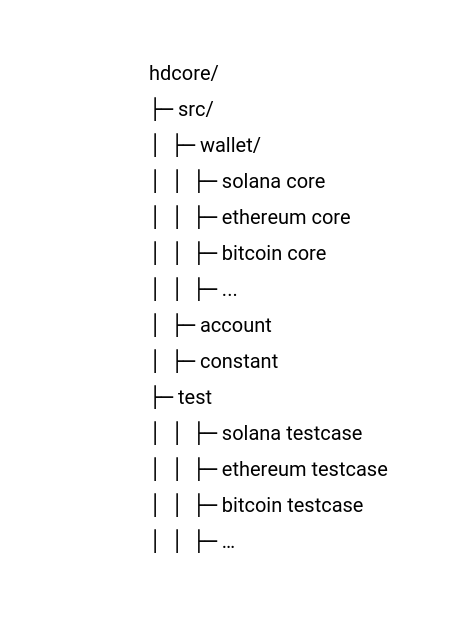
\includegraphics[width=0.5\textwidth]{images/lib_struct.png}
    \caption[General library structure]{General library structure}
    \label{fig:lib1}
\end{figure}

We name our library “hdcore” meaning the cores of HD wallets. The library is divided into two parts.

\begin{itemize}
    \item The /src folder comprises the /wallet folder which is the implementation of API for each chosen blockchain. There is also a constant file including all general information about the blockchain (index, url, etc. ). And an account file where we generalize the wallet folder, users can choose their blockchain wallet through this file.
    \item The /test folder contains test cases for every function.
\end{itemize}

\bigskip
{\textbf{API}}

The library will supports following features of a hd wallet:

\begin{itemize}
    \item Mnemonic code generation
    \item  Key pair generation
    \item Key tree derivation
    \item Address generation (for each blockchain)
    \item Verification of keys and addresses
    \item Balance checker
    \item Transaction builder (signing and broadcasting the transaction)
\end{itemize}


\bigskip
{\textbf{Unit testing}}

For testing our library, we use test vectors. A test vector offers a compact way of defining test input/output. It is a set of test cases where each test case is defined as a set of actions and expectations to verify our library's particular feature or functionality.

A test case contains steps as in \autoref{fig:testcase}. The test case includes specific variables or conditions, using which a user can compare expected and actual results to determine whether the library behaves appropriately as per their requirements.

\begin{figure}[ht!]
    \centering
    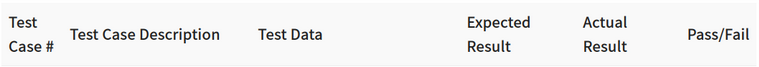
\includegraphics[width=0.8\textwidth]{images/testcase.png}
    \caption[Testcase components]{Testcase components}
    \label{fig:testcase}
\end{figure}

The test vector should show the functionalities of our library (declared in API).

\bigskip
{\textbf{Security}}

The library will acknowledge the security flaws, and we will look into this seriously. We focus on the coding concern, discussing how we can replace poisoned libraries, and prevent the addition of new vulnerable libraries to our code.

We discuss our properties from different perspectives:

\begin{itemize}
    \item Information leaking: Part of the API supports the connection to the blockchain (for broadcasting the transaction); therefore, we have to make sure the library would not send any sensitive or redundant information.
    \item Library implementation: We will carefully analyze the library dependencies if we choose to use them, even benchmarking them if necessary.
    \item Programming language: We will discuss the safety of the language we choose to implement.
\end{itemize}

Our library will be published to the related package manager, so open-source users and developers can audit and give us their thoughts.

\bigskip
{\textbf{Documentation}}

The goal of our documentation is an overview and usage exploration of our library. Thus, the documentation comprises all the expected results of the main functions, overlook of test vectors, and how to apply to some specific blockchains.



\section{The Hierarchical Deterministic Web Wallet}
We decided to create a web wallet for our thesis so we don’t have to deal with version control and different kinds of operating systems (Android, iOS, etc.). Everybody can access our website with their browsers.

Our web wallet is a non-custodial hot wallet where users can sign in, generate accounts in different blockchains, and send and receive native tokens (see \autoref{fig:webwallet}). They have absolute controls over private keys for every blockchain address, and the wallet provider has no access to them. We will use the localhost environment as a server for the wallet provider.

\begin{figure}[ht!]
    \centering
    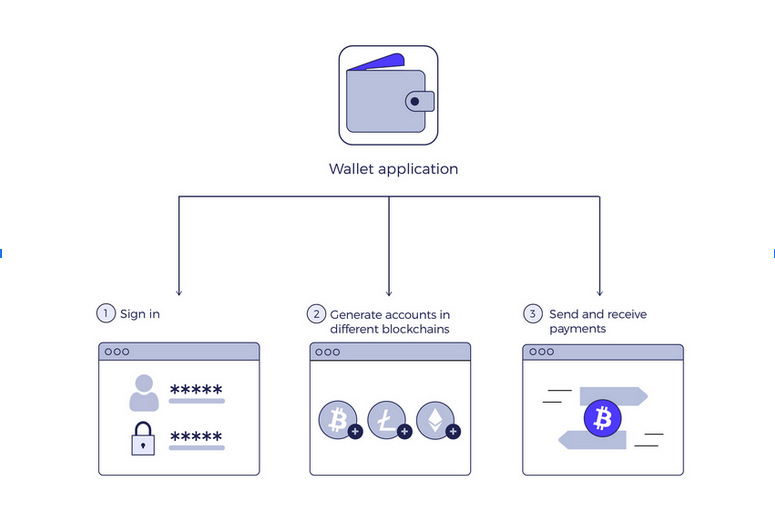
\includegraphics[width=0.8\textwidth]{images/webwallet.png}
    \caption[Example of Web Wallet flow]{Example of Web Wallet flow}
    \label{fig:webwallet}
\end{figure}

\subsection{Cryptographic mechanism}
The security of cryptography defines the strength of the blockchain wallet. Everything is protected by the laws of mathematics. We discuss which technology from Section [Ref technology] will be implemented for our wallet protocols.

\bigskip
{\textbf{Key pair and Address}}

In a blockchain system, the private key determines the ownership of the address property generated by the corresponding public key. Our generated key pair must be corresponding to each other. The private key is required to be functioned appropriately when the owner accesses and sends cryptocurrency. The address is an encoded or produced by cryptographic algorithm from the public key depending on the Blockchain cryptographic system. Our wallet addresses can be looked up on network explorers.

We will support Solana and Ethereum blockchain which utilises secp256k1 and ed25519.

\bigskip
{\textbf{Password generation}}

A password or a mnemonic code is the secret that users have to back up and keep away from the internet. From the code, users can recover the whole wallet tree from a single seed due to all the keys of a wallet being derivable from a single plaintext string. With this property, even key transfer and management are very convenient. We will implement BIP39's mnemonic sentence process for our wallet since it is the industrial standard for seed wallets.
The architecture of the password generation is described in \autoref{bip39}.

\bigskip
{\textbf{Digital signature generation}}

We use both secp256k1 and ed25519 digital signature algorithms to sign our wallet’s transactions.

\bigskip
{\textbf{Key derivation}}

Derivation function is the most important part of our wallets. We presented three of the most famous schemas in Chapter \ref{chap: Related works}. In order to match the standard of cryptography technology to achieve a securely appropriate application, we will adapt hardened key derivation of both BIP32 (for secp256k1) and SLIP10 (for ed25519) for our wallet.
Our key derivation tree will look like \autoref{fig:webwallettree}

\begin{figure}[ht!]
    \centering
    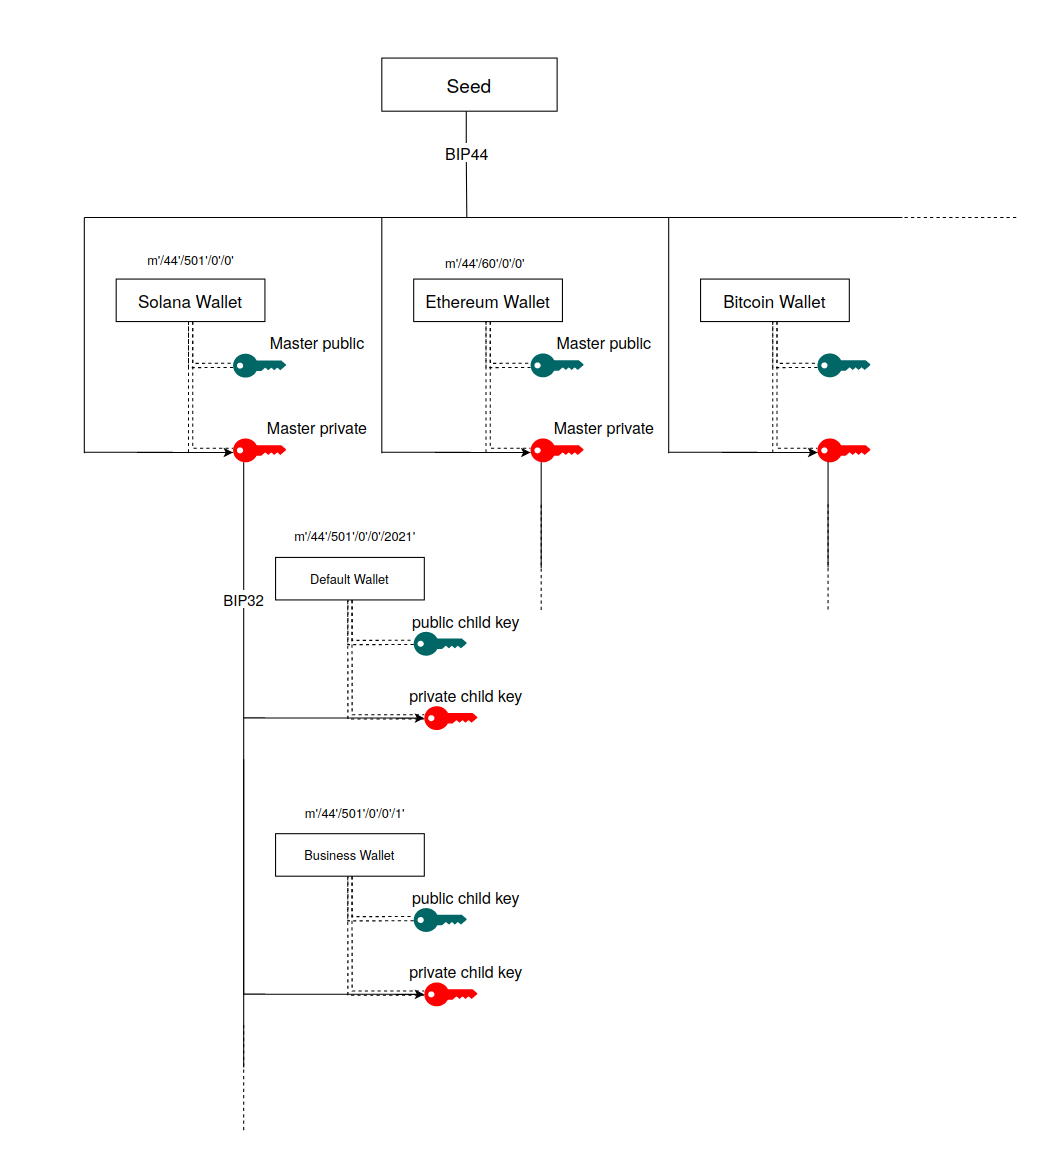
\includegraphics[width=1\textwidth]{images/tree_web_wallet.png}
    \caption[HD Web Wallet tree]{HD Web Wallet tree}
    \label{fig:webwallettree}
\end{figure}

The BIP32-ED25519 and normal key derivation of BIP32 have serious security flaws, as we explained in Section \ref{bip32vul}. Furthermore, the schema of public key derivation is only applicable to cold wallets where your private keys can be kept in a disjoint hardware while the master public keys can be broadcast to the internet.

\begin{adjustwidth}{1cm}{}

    \bigskip
    {\textbf{Solving the normal key derivation problem}}

    By applying the hardened key version, we will lose the magical ability of public key derivation. With the effort of optimizing the wallet, we came up with an idea that can replace this advantage. First, we discuss the disadvantages of BIP32 normal key derivation in our multicoin wallet:

    \begin{itemize}
        \item It still has serious flaws, as we mentioned (Section \ref{bip32vul}). All of the public key derivation systems will suffer this problem. Users cannot afford to give or lose any child keys since the attackers can recover the entire purse. Therefore cannot use this schema for any business operations.

        \item Users have to generate every master public key for every supported curve. For example, we support ed25519 and secp256k1, and our wallets will produce two different master public keys (\textit{mpub}) for two curves. Somebody who wants to send coins to us will have to save our two \textit{mpub}, look for the \textit{mpub} of a specific currency, generate the child address, and then ship the coins plus the index to that child. This restricts the scalability of our wallets if we're going to support more blockchain. It also affects users' experience if they have more connections (more \textit{mpub} to save).Our idea is explained as follow:
              We create a server to retrieve all the allowed addresses from our user wallets and store it as a tree structure. We call it “Address service” (details in Section [Ref ]). The purpose of this is to recreate the process of public key generation but in a more convincing way. Senders can perform an address look-up on the server to get the receiver’s currency address.

    \end{itemize}

    Our idea is explained as follow:
    We create a server to retrieve all the allowed addresses from our user wallets and store it as a tree structure. We call it “Address service” (details in Section \ref{system_architect}). The purpose of this is to recreate the process of public key generation but in a more convincing way. Senders can perform an address look-up on the server to get the receiver’s currency address.

    \begin{itemize}
        \item The server only holds customer addresses. The tree structure helps to optimize address searching.
        \item The server has no access to user transactions and assets. Users broadcast transactions straight to the blockchain network. The decentralized nature remains for our wallet.
        \item Private keys are still in control of user browsers.
    \end{itemize}

    The advantages of the server are listed as follow:

    \begin{itemize}
        \item Avoid the flaws of the BIP32 public key derivation completely.
        \item Senders only need to know one master public key of the receiver for the first time.
        \item Users have complete control of what wallet they want to show the internet. In BIP32 normal key derivation, if others have your master public key, they can generate the whole wallet public keys.
        \item Other users can't figure out the index of other wallets since there are only addresses in the server's database.
    \end{itemize}

    Also, since the server holds no sensitive information, the attacks aimed to spoof the user’s network (MITM attack \cite{mitm}) are useless.

\end{adjustwidth}



\subsection{System Architecture}
\label{system_architect}

\subsubsection{User and Web Service}

In practice, our system requires a server to host the RESTful web service to handle the requests from users. Users can access our wallet interface through their browser by entering the domain of our hosting service.

The protocols between users and our server describes as \autoref{fig:uws}:

\begin{figure}[ht!]
    \centering
    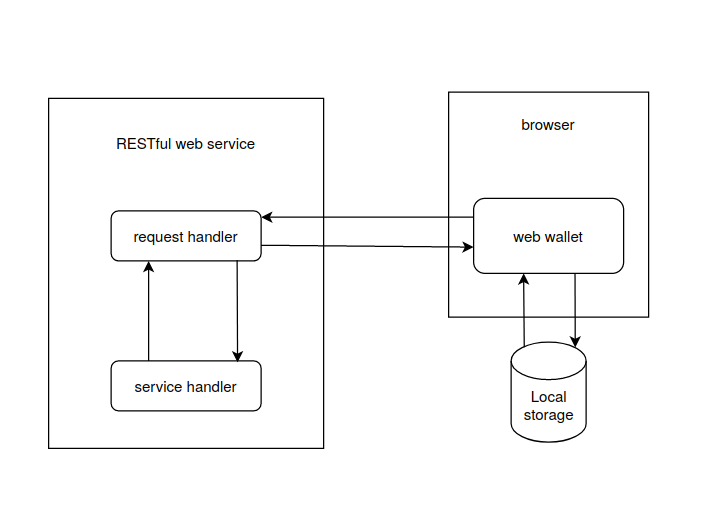
\includegraphics[width=0.8\textwidth]{images/design_uws.png}
    \caption[Between users and Wallet Provider]{Between users and Wallet Provider}
    \label{fig:uws}
\end{figure}

The server-side contains the request handler and service handler. The request handler acts like an endpoint where users send in their requests. Then parse the parameter and transfer it to the service handler. The service handler will read the information and return the content of the webpage (HTML, scripts, etc. ) to the users.

The client-side (user browser) accesses the wallet through a GET request to the server. All users' critical information will be saved at their local storage, like master private keys or passwords and they should be encrypted.

\subsubsection{User and Blockchain}

If the users want to make a transaction they will connect directly to the blockchain networks. Before building a transaction, users will decrypt the private key from their local storage. The private key will be used to sign the transaction. The transaction will be broadcast directly to decentralized networks without going through the server.

The protocols described as \autoref{fig:ubl}:

\begin{figure}[ht!]
    \centering
    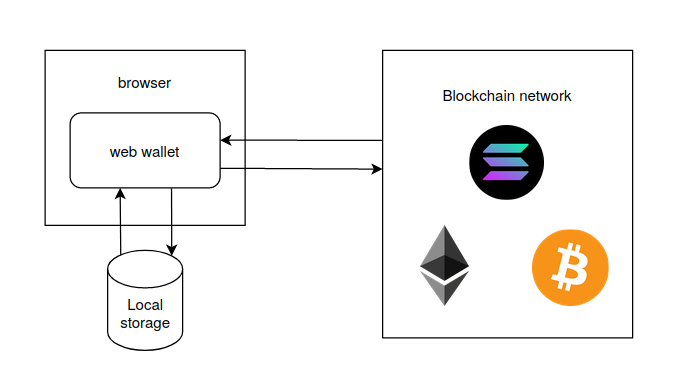
\includegraphics[width=0.8\textwidth]{images/design_ubl.png}
    \caption[Between users and Blockchain network]{Between users and Blockchain network}
    \label{fig:ubl}
\end{figure}

\subsubsection{User and Address Service}

We created another server to handle “Address service”. Note that we can combine this server with the Web Service Server above. But they served different purposes, and we don’t want our system to be synthetic. Furthermore, this separated architecture will be easier to update and test.

\begin{figure}[ht!]
    \centering
    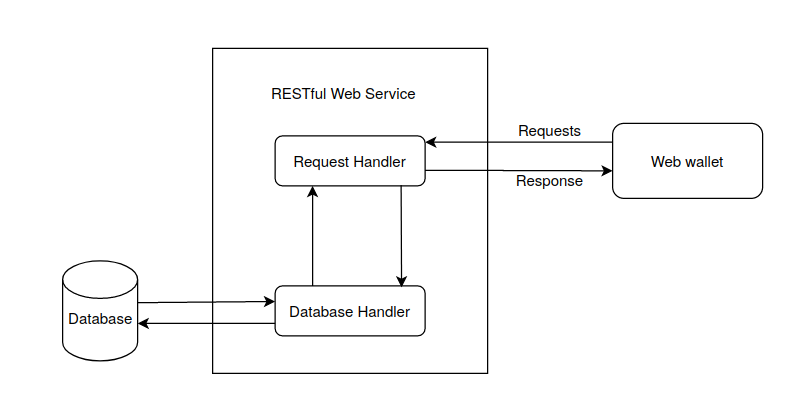
\includegraphics[width=0.8\textwidth]{images/design_uas.png}
    \caption[Between users and Address Service]{Between users and Address Service}
    \label{fig:uas}
\end{figure}

The users after creating their wallet will create a POST request to the server with their automatically created public keys in JSON.
The JSON data contains the address of master wallet and default child wallets.
We created the term "default child" just for init the hierarchical tree.
The struct of the JSON request present as Figure~\ref{fig:json}.

\begin{figure}[ht!]
    \centering
    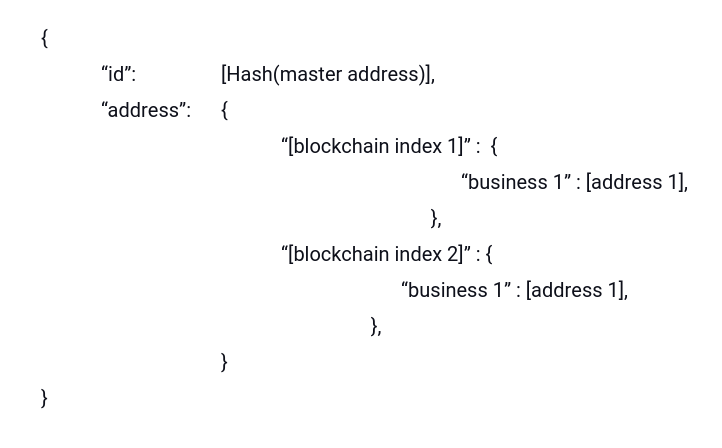
\includegraphics[width=0.9\textwidth]{images/design_json.png}
    \caption[Request Data]{Request Data}
    \label{fig:json}
\end{figure}

The database handler will save the JSON object from the request handler. The reason we choose the JSON object is that it is easier to be updated by the users. Furthermore, they are optimized by the search engine. We recommended using a NoSQL database program for this architecture, especially the one that utilized collections and documentations.

The database is designed just like the JSON object, but holds more values (see \autoref{fig:json1})

\begin{figure}[ht!]
    \centering
    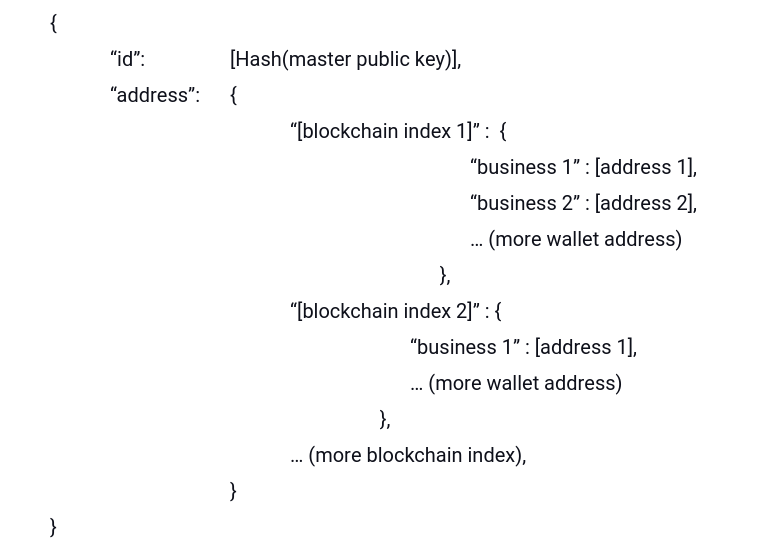
\includegraphics[width=0.9\textwidth]{images/json1.png}
    \caption[General JSON object of a Wallet]{JSON object of a Wallet}
    \label{fig:json1}
\end{figure}


\subsection{Information Privacy and Security concern}

Our browser-based crypto wallets give users complete control of their keys and therefore their funds. We guarantee the reliability of the website and the system behind it. The web provider will not hold any sensitive information or require any of the user's identification. On the other hand, the user needs to protect their secret and the hardware (or other place) where they keep them. In extreme cases, for example, the attacker takes over the user's computer (anything they access the wallet with), we can't do anything about it.

To design a web application with a priority on system security, we decided to take OWASP as a recommendation for yielding the foundation. OWASP is a non-profit global association that intends to promote application security across the web. It emerged as a standard awareness documentation for developers and web application security. OWASP strives to improve software security through its participating knowledge, open-source projects, material related, and thousands of community members. A security testing experiment will be done after we based on OWASP's top security risks that can be related to our project in Section . From high to low risk, they are:

\begin{enumerate}
    \item Broken Access Control.
    \item Cryptographic Failures.
    \item Injection.
    \item Insecure Design.
    \item Vulnerable and Outdated Components.
\end{enumerate}

The security tests will be examined with specific aims and different tools. We will try to cover all security threats in our system or at least protect our wallet from common security holes that can directly harm the end users.


\subsection{Use Cases}

\subsubsection{Use Case diagram}

\begin{figure}[ht!]
    \centering
    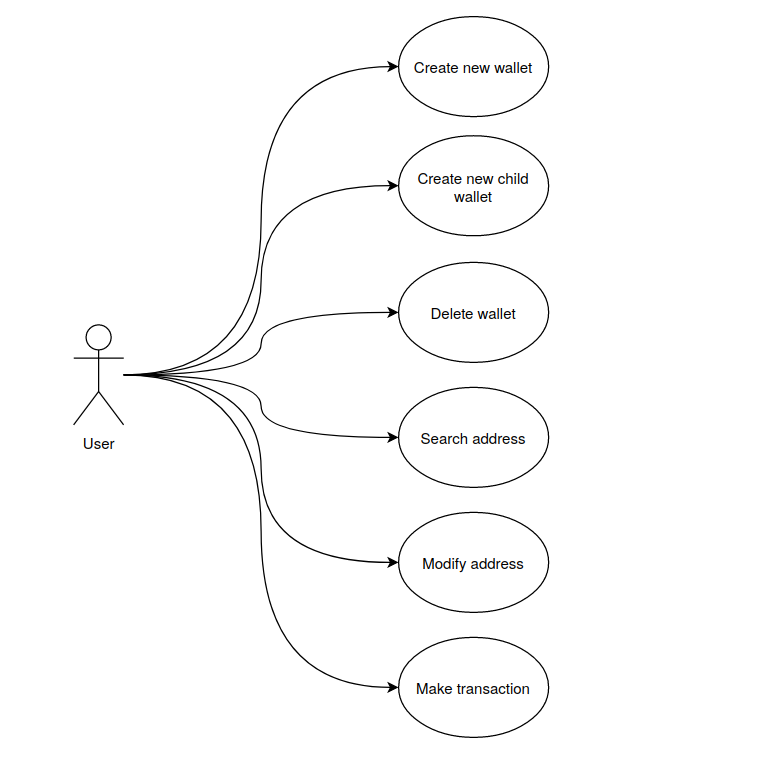
\includegraphics[width=1\textwidth]{images/usecases.png}
    \caption[General JSON object of a Wallet]{JSON object of a Wallet}
    \label{fig:usecases}
\end{figure}

\newpage
\subsubsection{Use case table}

\bigskip
{\textbf{Use case detail}}

\begin{table}[b]
    \begin{tabular}{| m{8cm} | m{6cm} |}
        \hline
        Use case name            & Table reference      \\ \hline
        Create new wallet.       & Table \ref{Tab:UC-1} \\ \hline
        Create new child wallet. & Table \ref{Tab:UC-2} \\ \hline
        Delete wallet.           & Table \ref{Tab:UC-3} \\ \hline
        Search address.          & Table \ref{Tab:UC-4} \\ \hline
        Modify address.          & Table \ref{Tab:UC-5} \\ \hline
        Make transaction.        & Table \ref{Tab:UC-6} \\ \hline
        % Share. & Table \ref{Tab:UC-8}\\ \hline
        % Set permission. & Table \ref{Tab:UC-9}\\ \hline
        % View change history. & Table \ref{Tab:UC-10}\\ \hline
        % Revert. & Table \ref{Tab:UC-11}\\ \hline
    \end{tabular}
    \captionof{table}{\label{Tab:UCList}Use case List}
\end{table}

\begin{table}[]
    \begin{tabular}{| m{4cm} | m{11cm} |}
        \hline
        Use Case Name:     & Create new wallet.                                                                    \\ \hline
        Event:             & The user accesses the wallet page.                                                    \\ \hline
        Description:       & The user chooses to create or recover their HD wallet and go on to their wallet page. \\ \hline
        Preconditions:     & \begin{itemize}
            \item Application has an internet connection.
        \end{itemize}                                                            \\ \hline
        Post-conditions:   & \begin{itemize}
            \item Default wallets are generated for the user.
            \item The user gets to their wallet page.
            \item The user is able to perform actions with their wallets.
        \end{itemize}                                                            \\ \hline
        Normal flows:      & \begin{enumerate}
            \item The user accesses the homepage from the browser.
            \item Web shows two options: “Create new wallet” and “Recover wallet”.
            \item Users choose “Create new wallet”.
            \item Web shows 12 or 24 mnemonic words.
            \item The user clicks on the create wallet button or refreshes the mnemonic code until they are satisfied with the code.
        \end{enumerate}                                                            \\ \hline
        Alternative flows: & \begin{itemize}
            \item {3a. TThe user chooses “Recover wallet”.}
                  \begin{itemize}
                      \item 3a.1. Web shows an input form.
                      \item 3a.2. Users enter their mnemonic code.
                  \end{itemize}
        \end{itemize}                                                            \\ \hline
        Exception:         & \begin{itemize}
            \item {3a. The user enters an invalid mnemonic code.}
                  \begin{itemize}
                      \item Web warns the users and tells them to enter another code.
                  \end{itemize}
        \end{itemize}                                                            \\ \hline
    \end{tabular}
    \captionof{table}{\label{Tab:UC-1} Use case: Create new wallet.}
\end{table}

\begin{table}[]
    \begin{tabular}{| m{4cm} | m{11cm} |}
        \hline
        Use Case Name:     & Create new child wallet.                                                  \\ \hline
        Event:             & The user chooses “Derive wallet” button to create a new child wallet.     \\ \hline
        Description:       & The user chooses to derive a new child wallet from the chosen blockchain. \\ \hline
        Preconditions:     & \begin{itemize}
            \item Application has an internet connection.
            \item The user already accesses the wallet page.
        \end{itemize}                                                \\ \hline
        Post-conditions:   & \begin{itemize}
            \item A child wallet is generated for the user.
            \item The user is able to perform actions with their child wallet.
        \end{itemize}                                                \\ \hline
        Normal flows:      & \begin{enumerate}
            \item The user chooses a blockchain on the top bar.
            \item Web shows that blockchain wallet page.
            \item The user chooses “Derive wallet” button.
            \item Web shows index input form.
            \item The user enters the index for the child wallet and click "Create".
            \item Web shows the child wallet.
        \end{enumerate}                                                \\ \hline
        Alternative flows: & N $\backslash$ A                                                          \\ \hline
        Exception:         & \begin{itemize}
            \item {5. The user enters an invalid index.}
                  \begin{itemize}
                      \item Web warns the users and tells them to enter another index.
                  \end{itemize}
        \end{itemize}                                                \\ \hline
    \end{tabular}
    \captionof{table}{\label{Tab:UC-2} Create new child wallet.}
\end{table}


\begin{table}[]
    \begin{tabular}{| m{4cm} | m{11cm} |}
        \hline
        Use Case Name:     & Delete Wallet from the browser.                                                                  \\ \hline
        Event:             & The user chooses “Delete this wallet” in the top bar.                                            \\ \hline
        Description:       & The user no longer uses the wallet and wants to delete the wallet information on their computer. \\ \hline
        Preconditions:     & \begin{itemize}
            \item Application has an internet connection.
            \item The user already accesses the wallet page.
        \end{itemize}                                                                       \\ \hline
        Post-conditions:   & \begin{itemize}
            \item Delete all local storage and session from the user browser.
        \end{itemize}                                                                       \\ \hline
        Normal flows:      & \begin{enumerate}
            \item The user clicks on “Delete this wallet”.
            \item Web warns the user if they are sure.
            \item The user chooses “Yes”.
            \item Web shows index input form.
            \item Web delete all information from user's local storage and browser session.
            \item Return to homepage.
        \end{enumerate}                                                                       \\ \hline
        Alternative flows: & \begin{itemize}
            \item {3. The user chooses “No”.}
                  \begin{itemize}
                      \item Web returns to the current stage.
                  \end{itemize}
        \end{itemize}                                                                       \\ \hline
        Exception:         & N $\backslash$ A                                                                                 \\ \hline
    \end{tabular}
    \captionof{table}{\label{Tab:UC-3} Delete Wallet from the browser.}
\end{table}


\begin{table}[]
    \begin{tabular}{| m{4cm} | m{11cm} |}
        \hline
        Use Case Name:     & Search address.                                                                                                                         \\ \hline
        Event:             & A bar pops up when the user clicks “Send” on the wallet component. To search for an address in the database, the user clicks “Look up”. \\ \hline
        Description:       & The user want to make a transaction and look up the receiver address of a blockchain.                                                   \\ \hline
        Preconditions:     & \begin{itemize}
            \item Application has an internet connection.
            \item The user already accesses the wallet page.
        \end{itemize}                                                                                                              \\ \hline
        Post-conditions:   & \begin{itemize}
            \item Return the receiver addresses of the chosen blockchain.
        \end{itemize}                                                                                                              \\ \hline
        Normal flows:      & \begin{enumerate}
            \item The user clicks on “Send” of a specific wallet.
            \item Web pop up a transaction box.
            \item The user fills in the master address of the receiver.
            \item Web returns a list of addresses of the receiver.
        \end{enumerate}                                                                                                              \\ \hline
        Alternative flows: & N $\backslash$ A                                                                                                                        \\ \hline
        Exception:         & \begin{itemize}
            \item {4. The address doesn't exist in the database, the web return zero address.}
        \end{itemize}                                                                                                              \\ \hline
    \end{tabular}
    \captionof{table}{\label{Tab:UC-4} Search address.}
\end{table}



\begin{table}[]
    \begin{tabular}{| m{4cm} | m{11cm} |}
        \hline
        Use Case Name:     & Modify addresses in the database (push or pull).               \\ \hline
        Event:             & The user clicks on “Pull" or “Push” from the wallet component. \\ \hline
        Description:       & The user chooses which wallet to public to others.             \\ \hline
        Preconditions:     & \begin{itemize}
            \item Application has an internet connection.
            \item The user already accesses the wallet page.
        \end{itemize}                                     \\ \hline
        Post-conditions:   & \begin{itemize}
            \item The chosen wallet address is either deleted or added in the database.
        \end{itemize}                                     \\ \hline
        Normal flows:      & \begin{enumerate}
            \item The user clicks on “Pull wallet”.
            \item The web shows requests succeed and status removed from database.
        \end{enumerate}                                     \\ \hline
        Alternative flows: & \begin{itemize}
            \item {1a. The user clicks on “Add”.}
                  \begin{itemize}
                      \item The web shows requests succeed and status added.
                  \end{itemize}
        \end{itemize}                                     \\ \hline
        Exception:         & N $\backslash$ A                                               \\ \hline
    \end{tabular}
    \captionof{table}{\label{Tab:UC-5} Modify addresses in the database.}
\end{table}


\begin{table}[]
    \begin{tabular}{| m{4cm} | m{11cm} |}
        \hline
        Use Case Name:     & Make transaction.                                    \\ \hline
        Event:             & The user clicks on “Send” from the wallet component. \\ \hline
        Description:       & The user wants to send coins to somebody.        .   \\ \hline
        Preconditions:     & \begin{itemize}
            \item Application has an internet connection.
            \item The user already accesses the wallet page.
        \end{itemize}                           \\ \hline
        Post-conditions:   & \begin{itemize}
            \item The coins is sent and the transaction is public to the blockchain explorer.
        \end{itemize}                           \\ \hline
        Normal flows:      & \begin{enumerate}
            \item The user clicks on “Send”.
            \item Web pop up a transaction box.
            \item The user enters the address of the receiver (by looking up or entering straight to the forms) and clicks “Confirm”.
            \item Web shows transaction status and link to blockchain explorer.
        \end{enumerate}                           \\ \hline
        Alternative flows: & N $\backslash$ A                                     \\ \hline
        Exception:         & \begin{itemize}
            \item {Web shows something wrong with the transaction and returns to the current stage.}
        \end{itemize}                           \\ \hline
    \end{tabular}
    \captionof{table}{\label{Tab:UC-6} Make transaction.}
\end{table}

\newpage
